\chapter{Evaluation}
\label{chap:evaluation}

%%%%%%%%%%%%%%%%%%%%%%%%%%%%%%%%%%%%%%%%%%%%%%%%%%%%%%%%%%%%%%%%%%%%%%%%%%%%%%%%%%%%%%%%%%%%%%%%%%%%

A number of experiments were conducted to evaluate the correctness of the implemented robot control system. The robot control system was ran in its entirety on a high-end machine running Ubuntu Linux 12.04 LTS. Specifically, the machine has an \emph{Intel Core i7 3770K} clocked at \emph{4.5Ghz} paired with \emph{16GB} of memory. An attempt to run the control system on an \emph{Apple MacBook Pro} was made, which has an \emph{Intel Core i5 3239M} clocked at \emph{2.6Ghz} paired with \emph{8GB} of memory, but the machine could not achieve the performance necessary for good operation.

\begin{figure}[!h]
	\centering
	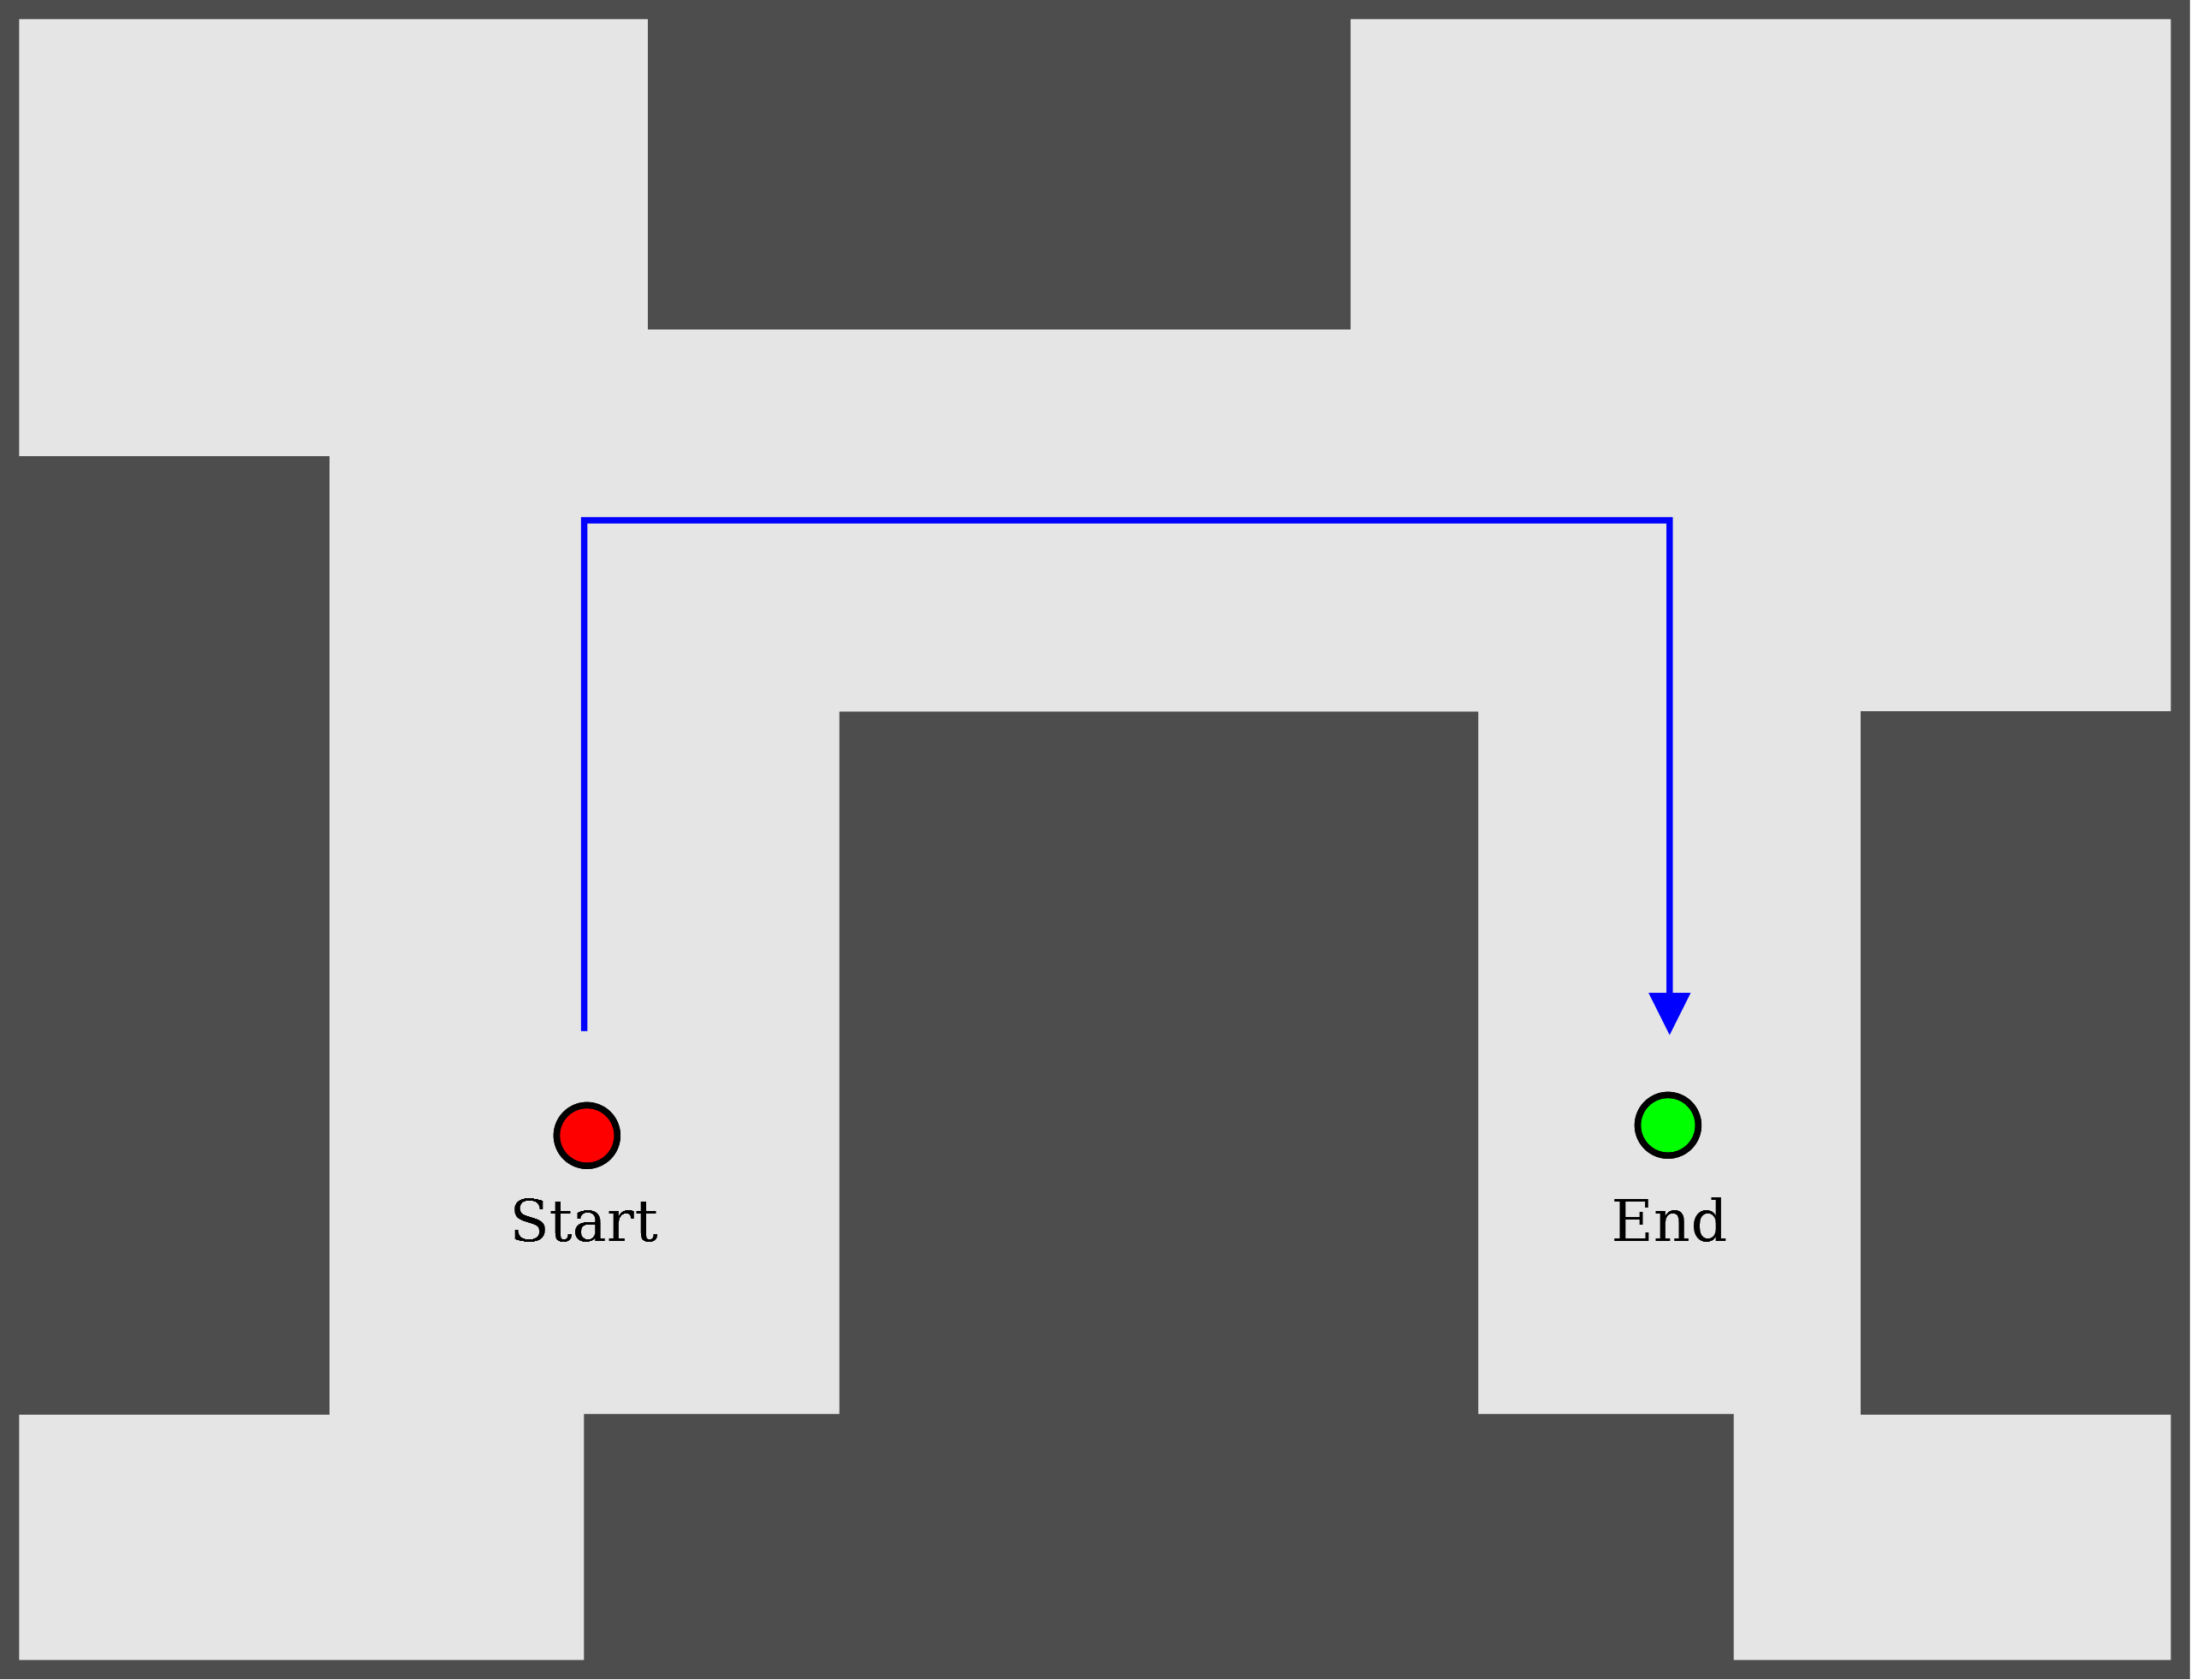
\includegraphics[width=12cm]{plan.png}
	\caption{A diagram of the general layout of the test environment (not to any particular scale). Darkened shapes indicate large obstacles that the robot must detect and avoid. The robot was placed at the starting point at the beginning of each test. The end point indicates the target goal for the navigational tests along with an ideal path.}
	\label{fig:eval_plan}
\end{figure}

Testing took place in a large environment as shown in \autoref{fig:eval_plan}. This environment contained a number of everyday obstacles with varying shapes, colours and textures. All tests were ran under ideal lighting conditions---i.e., full natural light---where possible. This ensured that the RGB-D sensor provided the highest quality images which would have a knock-on effect for the visual locomotory and mapping subsystems.

\section{Hardware Interaction}

These experiments were created to test the correct function of the hardware interaction systems, specifically the RGB-D camera driver and the servo driver.

\subsection{RGB-D Camera Driver}

The RGB-D camera driver, provided by the \texttt{openni2\_driver} and \texttt{openni2\_launch} packages, was tested by observing output through \emph{RViz}. A \emph{RViz} configuration was made that would show both the colour and depth video feeds from the camera, taken from the \texttt{/camera/color/image} and \texttt{/camera/depth/image} topics. As this is a standard package, it was expected that it would function as intended without any issues.

That said, a peculiar fault was discovered in that the device would show itself to be disconnecting and reconnecting repeatedly while running. Throughout this, many USB timeout messages and similiar errors were shown in the Linux \emph{message buffer} (shown by \texttt{dmesg}). The cause of the issue turned out to be that, simply, the USB cable from the computer to the camera was too long. The USB specification that devices running in USB 2.0 mode---which is the case for the \emph{Xtion}---may have a maximum cable length of $5$m \cite{usb_spec}. The cable had been extended to allow a larger movement distance but the resulting cable length was now $6.5$m long, as the \emph{Xtion} already had a $1.5$m cable attached.

Following this discovery, the cable was trimmed to $5$m and, as a result, the driver functioned correctly as intended.

\subsection{Servo Driver}

To test the servo driver for the system, which is implemented as a custom \texttt{servo\_controller} node, we ran the following experiments. Each experiment was implemented as a custom node would would then be ran alongside the driver nodes to execute the test. Correctness of results were determined by visual observation---i.e., looking to see if joints moved as intended. 

\subsubsection{Rotation of a Single Servo}

This first test was designed to confirm correct behaviour when moving only one servo at a time. To elaborate further, this test aimed to check the following:

\begin{description}[labelindent=\parindent]
	\item[Hardware Communication] \hfill \\
	If the servo controller was receiving any of the serial output sent by the \texttt{servo\_controller} node whatsoever, the on-board indication LED would flash with each message. This would have shown that the servo controller is receiving serial output as intended. No flashing LED would have indicated some general issue with the serial communication systems.

	\item[Topic Reception] \hfill \\
	If the \texttt{servo\_controller} node was receiving \texttt{ServoCommand} messages sent on its \texttt{direct} topic, we expected some sort of change in system state in general---even if that involved the node crashing. No change would have indicated a problem with the topic subscriber within the node.

	\item[Index, Angle \& Duration Conversion] \hfill \\
	Should the formulae from converting from the units specified in the \texttt{ServoCommand} message to those specified by the servo controller's protocol be correct, we would have expected the specified servo to move the correct angle over the correct duration. Any deviation from this would have indicated some mathematical error in the formulae.
\end{description}

To implement this test, a \texttt{servo\_controller\_test\_single} node was created. This node requests four movements from each servo sequentially in a continuous loop at various angles and durations, pausing for one second between each. A listing of these movements is shown in \autoref{tab:servo_controller_eval}.

\begin{table}[!h]
	\centering
	\begin{tabular}{ c c c }
		\toprule
		\textbf{Movement} & \textbf{Angle} & \textbf{Duration} \\
		\midrule

		$1$ &
		$90$\textdegree{} &
		$1.00$s \\

		$2$ &
		$180$\textdegree{} &
		$0.25$s \\

		$3$ &
		$0$\textdegree{} &
		$0.50$s \\

		$4$ &
		$90$\textdegree{} &
		$0.75$s \\
		\bottomrule
	\end{tabular}
	\caption{A listing of movements made for each servo in the single servo rotation test. These movements are applied to each servo in a continuous loop with a one second delay between each movement.}
	\label{tab:servo_controller_eval}
\end{table}

The \texttt{servo\_controller} node and \texttt{servo\_controller\_test\_single} node were launched and the robot observed. Prior to this, the robot was placed upon a pedestal to ensure that the limbs could rotate freely without unintentionally moving the robot. As expected, each servo rotated as intended to the correct angles and durations, thus showing the implementation was functional as required.

\subsubsection{Simultaneous Rotation of Multiple Servos}

The second test was designed to confirm correct behaviour in the case of multiple servos being moved simultaneously---i.e., in the case where movement is requested for a number of servos such that the movement durations overlap. This was an essential requirement as no walk gaits would be possible without.

To implement this test, the \texttt{servo\_controller\_test\_single} node from the previous test was adapted to create a new \texttt{servo\_controller\_test\_multiple} node. This node performed the same set of movements but on all servos simultaneously rather than sequentially.

The \texttt{servo\_controller} node and \texttt{servo\_controller\_test\_double} node were launched and the robot observed, while the robot was placed on a pedestal as before. It was from this test that the necessity for a small delay between each serial communication was discovered. Without this delay, servos would either not rotate whatsoever or abort their requested rotation part-way through. During this, the indication LED on the servo controlled would also light up solidly, rather than flash as it does during normal operation. It was presumed that this meant there was some sort of communication error, perhaps as commands were being sent too quickly for the on-board microcontroller to process them. After adding an delay of $0.1$s, the problem immediately subsided. This was further reduced to a minimum delay of $0.003$s by trial-and-error, preventing any knock-on effects for commanding nodes. As mentioned in the implementation section for the \texttt{servo\_controller} node, no source code is available for the microcontroller software so no further diagnosis can be made. 

Following this modification, the test ran as intended, thus showing the implementation was functional as required.

\section{Locomotion}

These experiments were created to evaluate that the systems designed to handle locomotion operated correctly. Specifically, we aimed to test the correct function of the limb controller, the limb calibration tool, and the walk controller.

\subsection{Limb Controller}

The limb controller, implemented as a custom \texttt{limb\_controller} node, was tested in a manner similar to the servo controller. The servo controller test nodes were adapted to send messages to the limb control topics, rather than the topic used to control the servos directly. Through running the same set of tests, the limb controller was shown to function correctly.

\subsection{Limb Calibration Tool}

The implementation of the limb calibration tool is fairly trivial and was used throughout the evaluation of the control system and as such, no particularly rigorous testing was performed. Testing was performed throughout the implementation process and the node was found to work as intended. Generally, the joint servos had to be re-calibrated during each session of operation, as the particular servos used are rather inaccurate. A number of realisations came about during its use.

In particular, it was found that achieving an accurate calibration through manual manipulation was essentially impossible. There are no markings on the robot with which the current angles of joints can be compared, so calibration was usually done by eye alone. Using a measuring implement, such as a protractor, was also infeasible as the physical geometry of the robot prevents such devices from aligning correctly with the servo axles. This issue could be alleviated by adding additional sensors on the robot---e.g., gyroscopes and accelerometers---such that calibration could be performed automatically or to, at the very least, give some notion of the stability of the robot.

Additionally, it was found that the servos would not rotate by small increments but only when it had reached a certain threshold away from its current position---e.g., if a servo is currently at $90$\textdegree{} then it will not rotate immediately until a rotation of $\pm2$\textdegree{} is requested whereupon it will ``snap'' into position. The particular threshold seemed to vary wildly depending on the particular servo \emph{and} its position. This ramifications of this were such that while a limb may seem calibrated, it could in fact be out of alignment by this threshold. This would only become apparent when larger rotations were made.

In general, both of these issues could be solved be utilising more accurate (and accordingly more expensive) servos---software can only correct for hardware problems up to a point.

\subsection{Tripod Gait Controller \& Gamepad Controller}

To test the tripod gait controller, implemented by the \texttt{gait\_controller} node, we conducted the following set of experiments. These would confirm that the implemented tripod gait cycle was correct and resulted in motions as intended. Specifically, we would test that the gait worked correctly for forward motions, angular motions and a combination of both motions. Manual control would be used throughout the test, given from the \texttt{gamepad\_controller}, providing confirmation that it was functioning correctly. Tests would involve observing the robot visually as it moved around.

\subsubsection{Linear Motion}

The first test involved simply moving the robot back and forth in a straight line from its starting position. The left analogue stick on the controller was pushed upwards and downwards, signifying a forward and backwards movement. This was done for a few minutes to ensure there were no problems. As expected, the robot moved as intended without issue.

\subsubsection{Angular Motion}

The second test involved rotating the robot in place. The right analogue stick on the controller was pushed left and right, signifying anti-clockwise and clockwise rotations. Again, this was done for a number of minutes to ensure that there were no problems. As expected, the robot rotated as intended.

\subsubsection{Combined Linear and Angular Motion}

The third test involved supplying commands for both linear and angular motions simultaneously, such that the robot would move in a curved path. This was essentially a combination of the previous two tests. Both the left and right analogue sticks on the controller were moved in varying combinations of positions. The expected outcome was that the robot should push forward while also turning to one side.

It was through this test that the necessity to apply some sort of equal ratio formula to the swing angles was found. Originally, both linear and angular movement angles were simply added together based on the requested velocities---i.e., $v_x \times \texttt{swing\_angle} + v_\theta \times \texttt{swing\_angle}$. This meant that both full linear and angular movements were requested, the resulting angles sent to the servos would be twice the specified maximum---i.e., $2 \times \texttt{swing\_angle}$. This was a rather nasty problem as it caused the legs of the robot to collide and get stuck inside one another.

The solution was to ratios such that the maximum angle sent to the servos could only be \texttt{swing\_angle}, as described in great detail in the implementation section. After applying this correction, the robot could move around correctly as intended. However, while this correction prevents the legs from colliding with one another, the speed at which the robot moves is somewhat reduced. If both maximum linear and angular movements are requested, the robot will only move at half the maximum speed, as the ratio formula divides \texttt{swing\_angle} equally.

\section{Sensing}

These experiments were created to evaluate that the systems could interpret the world around the robot via the supplied sensory input. Specifically, we test both the visual odometry and mapping systems.

\subsection{Visual Odometry}

To test the visual odometry system, which was provided by a \texttt{visual\_odometry} node in the \texttt{ccny\_rgbd} package, we ran the following experiments. These experiments involved moving the robot in various ways while observing how accurately the visual odometery system matched these movements. Experiments would be ran with both manual movement of the robot---i.e., lifting it up along a path by hand---as well as with the implemented tripod gait. The \texttt{tf\_echo} tool from the \texttt{tf} package was used to get an exact readout of the interpreted position. Each experiment was ran ten times and the resulting positions averaged.

\subsubsection{Linear Motion}

The first experiment involved moving the robot forward by one meter while observing the position given by the visual odometery system. At the start of each test, the robot was placed at the starting position shown in \autoref{fig:eval_plan} and the control system reset. The robot would then be moved forward---either manually by hand or via the tripod gait---such that the robot had moved a meter relative to this starting position. Two points were placed both at the start and end positions such that the front two feet could be aligned with them. An ideal result would have been a resulting position of $(1$m, $0$m, $0$\textdegree{}$)$.

By manual movement, the visual odometery system gave an average position of $(0.924$m, $0.004$m, $0.471$\textdegree{}$)$. Notably, the system seemed to underestimate the $x$ component by an average of $0.076$m in this case, while the $y$ component and heading remained fairly accurate. A full listing of the results can be seen in \autoref{tab:eval_vo}.

By movement via the tripod gait, the visual odometery system gave an average position of $(0.952$m, $0.013$m, $0.191$\textdegree{}$)$. Similarly, the system seemed to underestimate the $x$ component by an average of $0.048$m while the heading remains reasonably accurate. The higher $y$ component drift in this case could be due to the roughness of the walk gait. Specifically, the camera does not glide forward exactly in a straight line as it does when being moved manually through the air. Each step causes the robot shake in general as it settles into position. Again, a full listing of the results can be seen in \autoref{tab:eval_vo}.

\subsubsection{Angular Motion}

The second experiment involved rotating the robot by $90$\textdegree{} in place. As before, the robot was placed at the starting position shown in \autoref{fig:eval_plan} and the control system reset at the start of each test. The robot would then be rotated clockwise by 90\textdegree{} on the spot either either manually by hand or via the tripod gait. An ideal result would have been a resulting position of $(0$m, $0$m, $90$\textdegree{}$)$.

By manual movement, the visual odometery system gave an average position of $(0.1$m, $0.004$m, $89.296$\textdegree{}$)$. By movement via the tripod gait, the visual odometery system gave an average position of $(0.172$m, $-0.018$m, $89.284$\textdegree{}$)$. A full listing of the results from both tests can be seen in \autoref{tab:eval_vo_walk}.

In both cases, there was a significant drift in the $x$ component---a drift of $0.1$m and $0.172$m for the manual and tripod gait movements respectively---while the $y$ and $\theta_z$ components remained fairly accurate. While observing the visual odometry output through \emph{RViz}, it seemed as though the robot was rotating around a pivot rather than in place as it should be. This was a particularly troubling outcome as it had the potential to disrupt both the mapping and navigation systems, but no further diagnosis could be done without delving into the complexities of the node's source code. It is possible that a more in-depth calibration of the camera lenses is necessary, as any warping of points caused by the lens may not be taken into account. A further evaluation into this particular aspect is definitely necessary.

\subsubsection{General Commentary}

As an additional issue, should the visual odometry system be unable to find sufficient features in the images it is currently receiving---e.g., some object is obstructing the camera--- then the output positional will be essentially, undefined. While an actual position is output but the system, it could essentially be considered completely random and therefore useless. Additionally, when the system is able to find sufficient features once more, the position does not reset to where it was previously. At this point, the whole control system must be restarted.

In general, it is was not unexpected that the visual odometry system had some positional drift. The concept of odometry is such that it provides an estimate of the current position in space, rather than an exact position. Additional sensors---e.g., laser scanners, accelerometers, GPS, etc---would be very useful in this case. A multitude of filters can then be used to combine the information such that the robot can be localized in space much more accurately.

\subsection{Mapping}

To evaluate the mapping system, we ran the following set of tests. These tests would confirm that the mapping system could interpret the environment surrounding the robot correctly. Additionally, they would confirm that the map can update in real-time as the robot moves around the environment. A \emph{RViz} configuration was made to display both 2D and 3D maps generated by the \texttt{octomap\_server} node.

\subsubsection{Stationary Mapping}

The first test involved placing the robot on the starting position as shown in \autoref{fig:eval_plan}. The robot control system would then be started, and the map output shown in \emph{RViz} observed visually, checking the map for general accuracy versus the real environment. No movements---apart from putting the robot into a steady standing position---would be performed.

\begin{figure}[h]
	\centering
	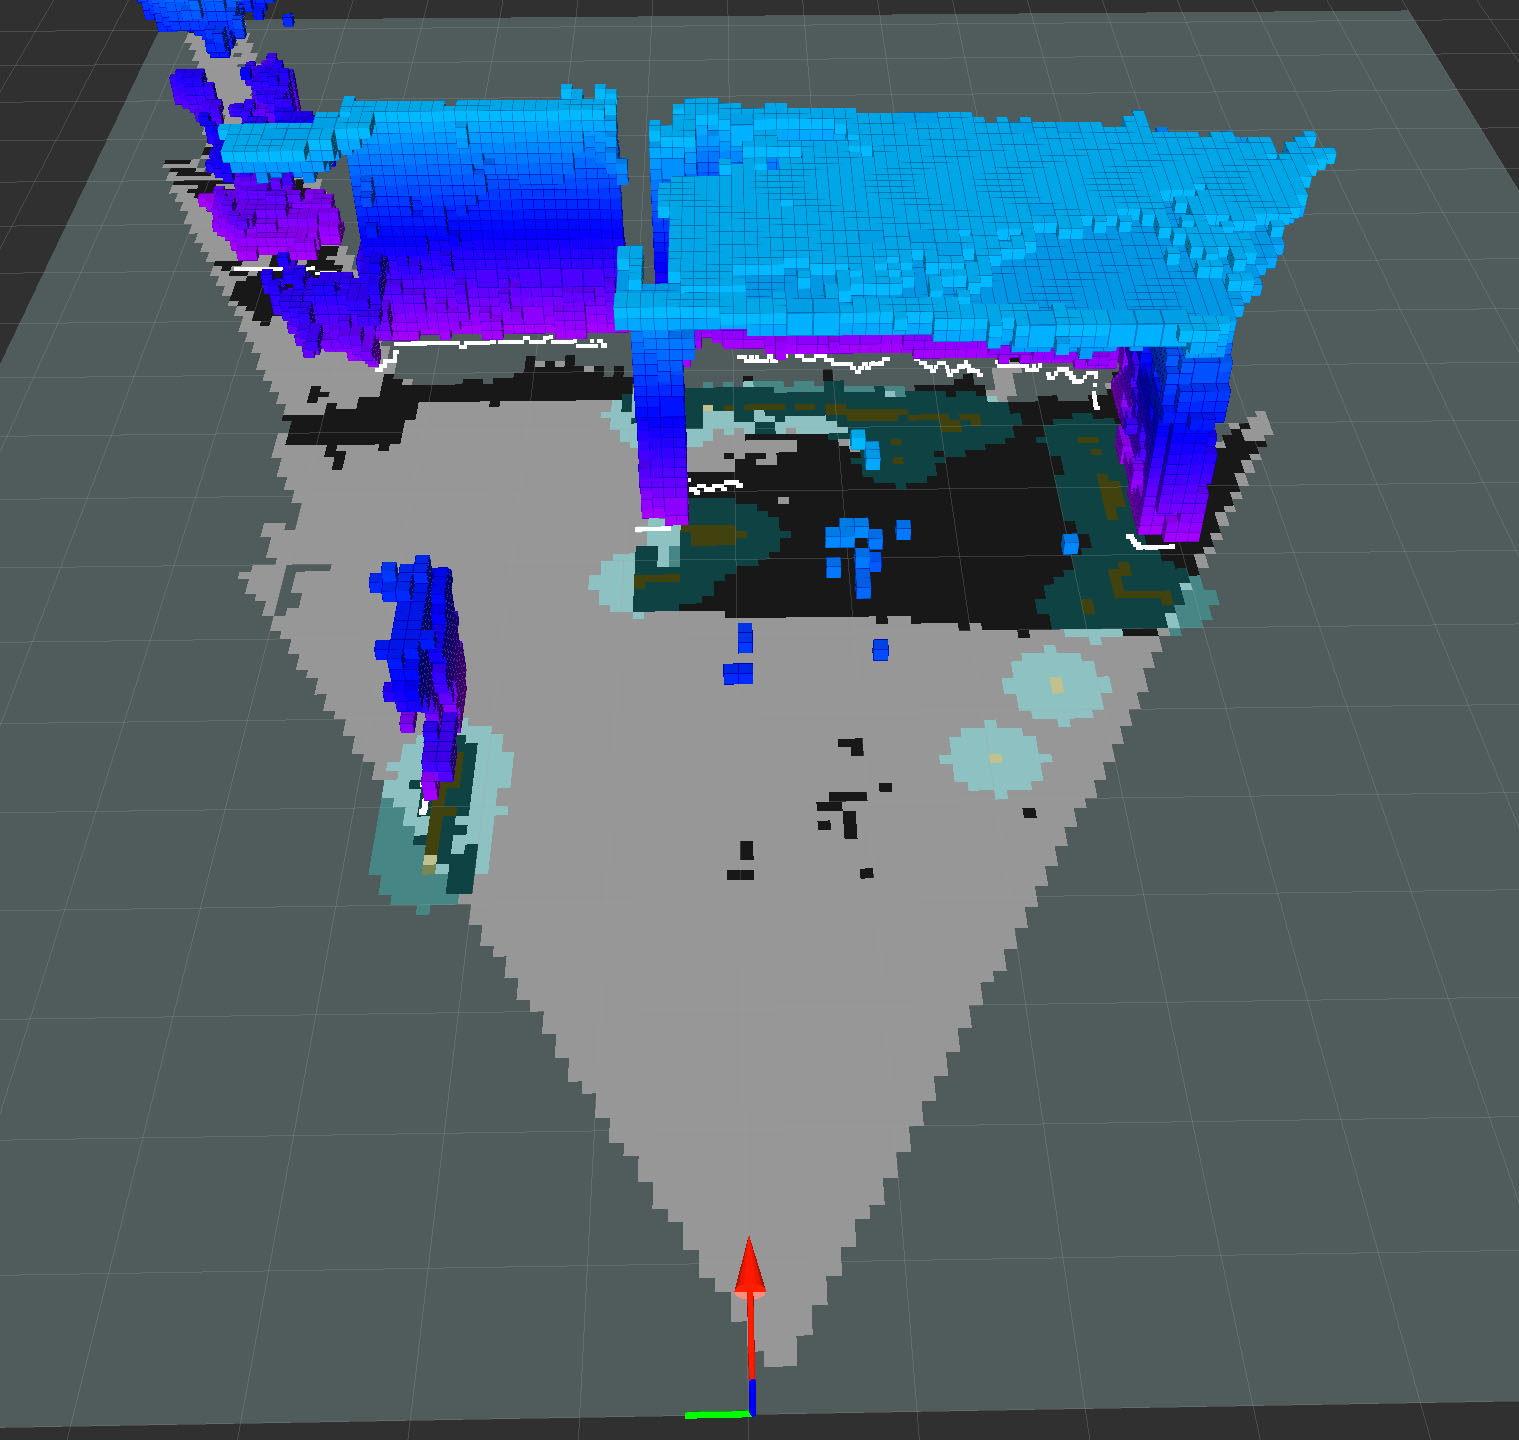
\includegraphics[width=14cm]{eval_map1.jpg} \\
	\vspace{2pt}
	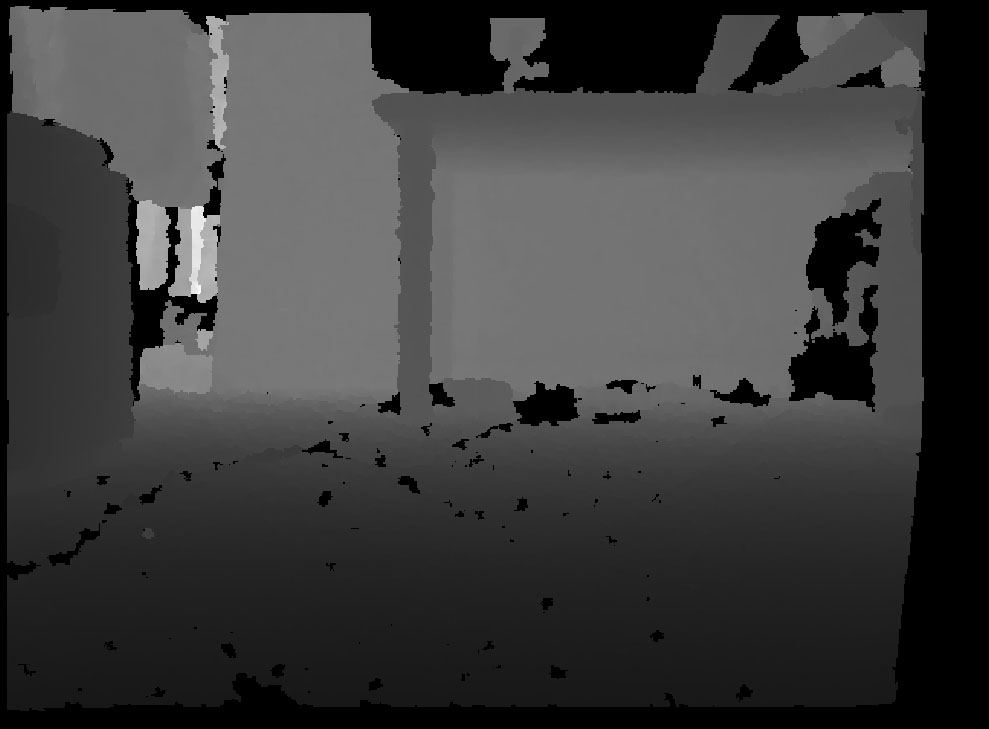
\includegraphics[width=8cm]{eval_rgbd3.jpg}
	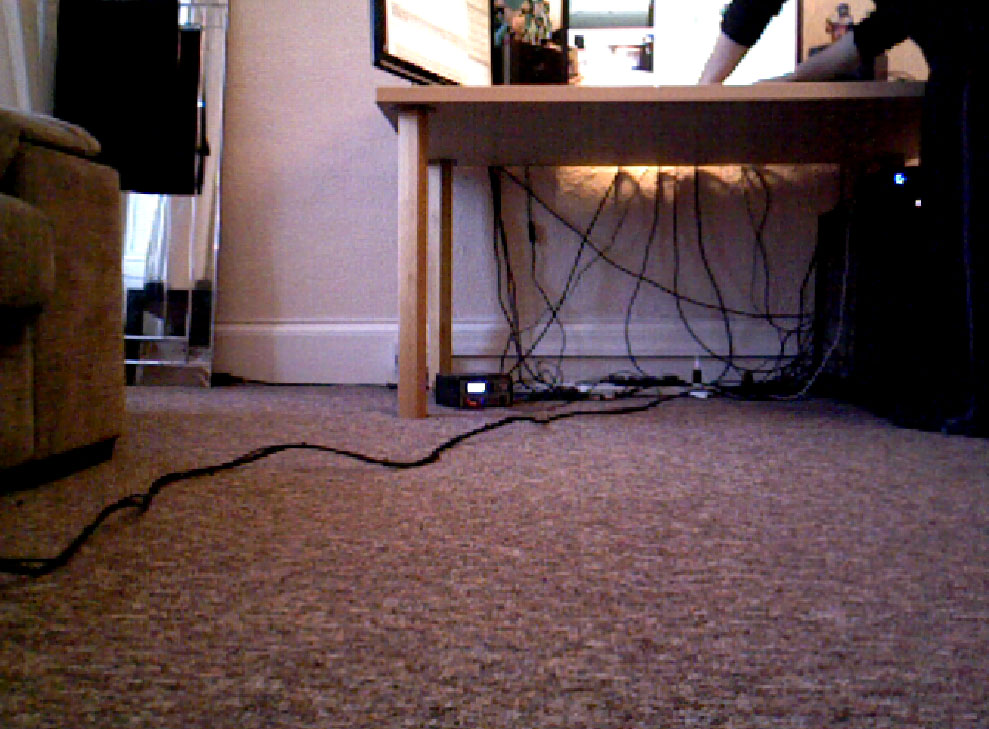
\includegraphics[width=8cm]{eval_rgbd4.jpg}
	\caption{A display of the generated map a few seconds after the robot control system has started along with the direct colour (bottom left) and depth (bottom right) outputs from the RGB-D camera. The shape of the desk and wall directly in front of the robot, as seen in the colour image, can clearly be seen in the resulting map.}
	\label{fig:eval_map_nobag}
\end{figure}

The resulting output along with raw imagery from the camera for this test as shown in \autoref{fig:eval_map_nobag}. While the map was generally accurate, there was some noise visible in the map output which is visible around the middle of the map output. It is possible that the mapping system could have erroneously detected some parts of the floor as obstacles. Regardless, they are so insignificant that the navigational systems would not have any issue with them. Thusly, this test was deemed successful.

\subsubsection{Stationary Mapping with an Obstacle}

The second test was performed in a manner similar to the previous test. At the start of the test, the robot was placed at the starting position and the control system started. The map output from the same \emph{RViz} configuration would then be observed. This time, however, after a few seconds an obstacle---in this case a backpack of similar height to the robot---would be placed $1$m in front of the robot. It was expected that the bag should then show up as an obstacle on the map. No movement would be performed, as before.

\begin{figure}[h]
	\centering
	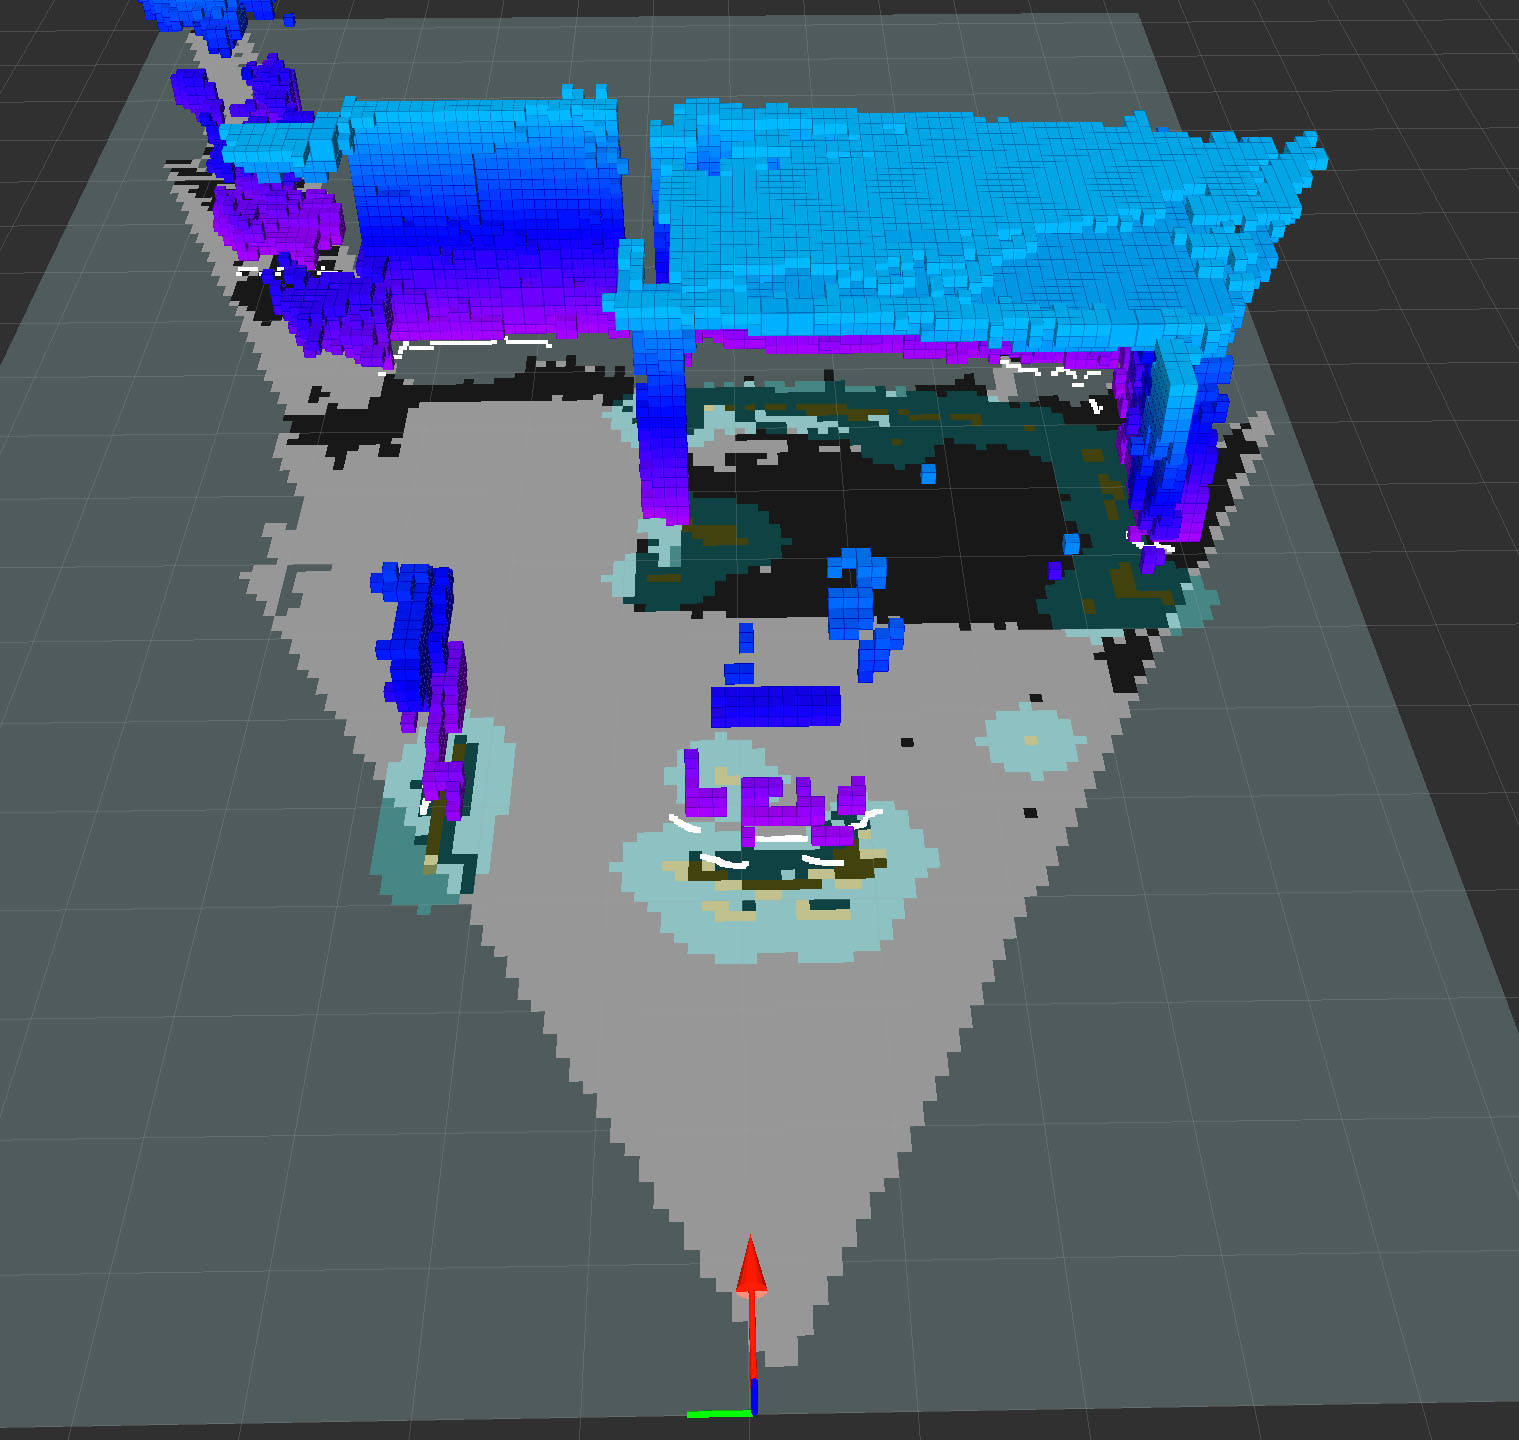
\includegraphics[width=14cm]{eval_map2.jpg} \\
	\vspace{2pt}
	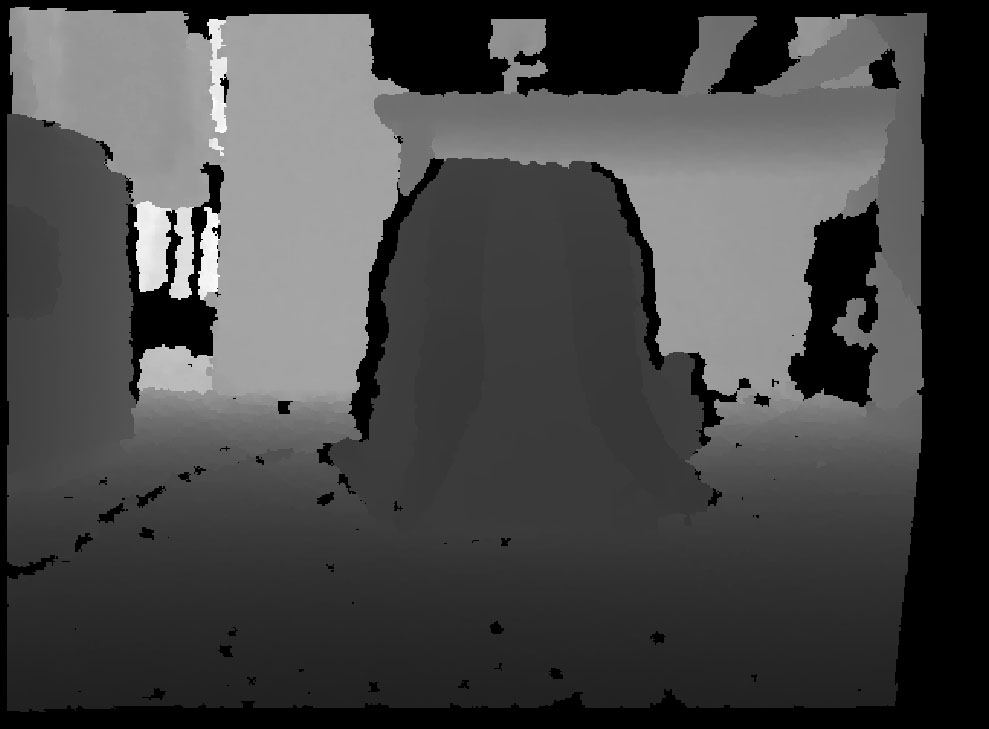
\includegraphics[width=8cm]{eval_rgbd1.jpg}
	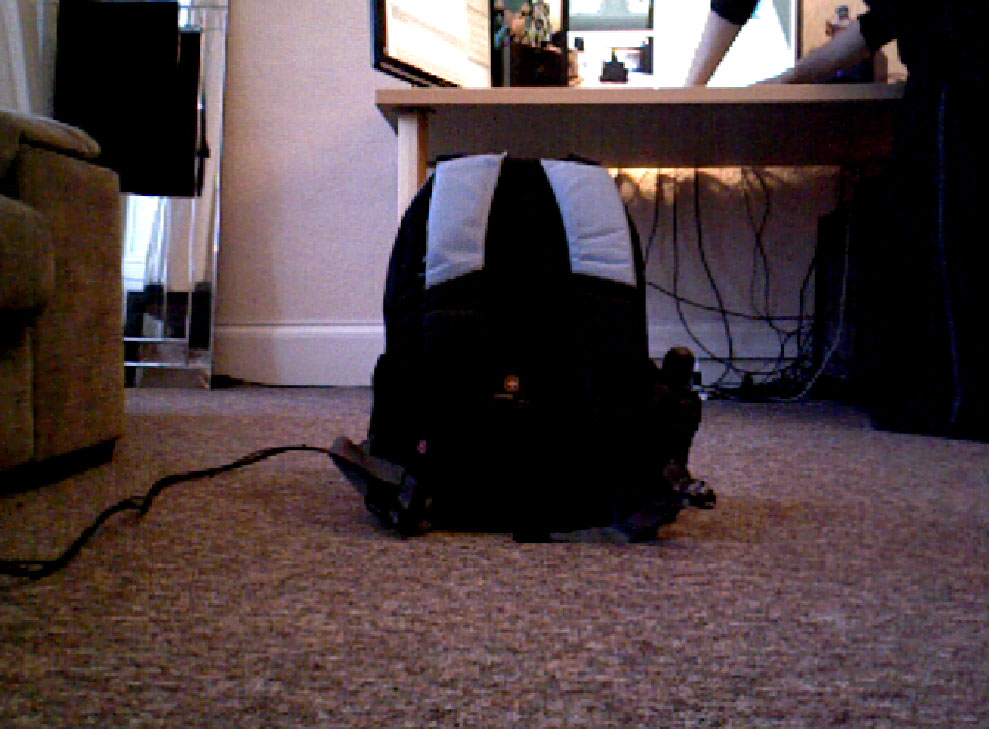
\includegraphics[width=8cm]{eval_rgbd2.jpg}
	\caption{A display of the generated map after an obstacle has been placed in front of the robot---a backpack in this case---along with the direct RGB (bottom left) and depth (bottom right) outputs from the RGB-D camera. The resulting blocks from the bag can be seen on the map. Notably, the bag appears as a rather patchy grouping of blocks but would still be enough to trigger any avoidance routines from the navigation system.}
	\label{fig:eval_map_bag}
\end{figure}

The resulting output after having placed the obstacle in front of the robot can be seen in \autoref{fig:eval_map_bag}. In this case, the surrounding environment was mapped quite accurately once again. The bag was also detected and mapped, however the resulting points were rather disjointed. The full shape of the obstacle was not mapped completely, even though it can be seen quite clearly in the raw imagery. Even though this was the case, the navigational system would have still been able to route around these points as the base footprint of the object can still be seen.

\subsubsection{Mapping During Walk Cycle}

The final test aimed to test the accuracy of the mapping system as the robot moved around the environment using the tripod gait. In particular, the robot would walk around the environment along the path as shown on \autoref{fig:eval_plan}, starting from the start position and ending at the end position. Manual control through the gamepad controller would be used for this test, rather than relying on the navigational system. The same \emph{RViz} configuration from previous tests would be used to visually observe the generated map for accuracy.

\begin{figure}[h]
	\centering
	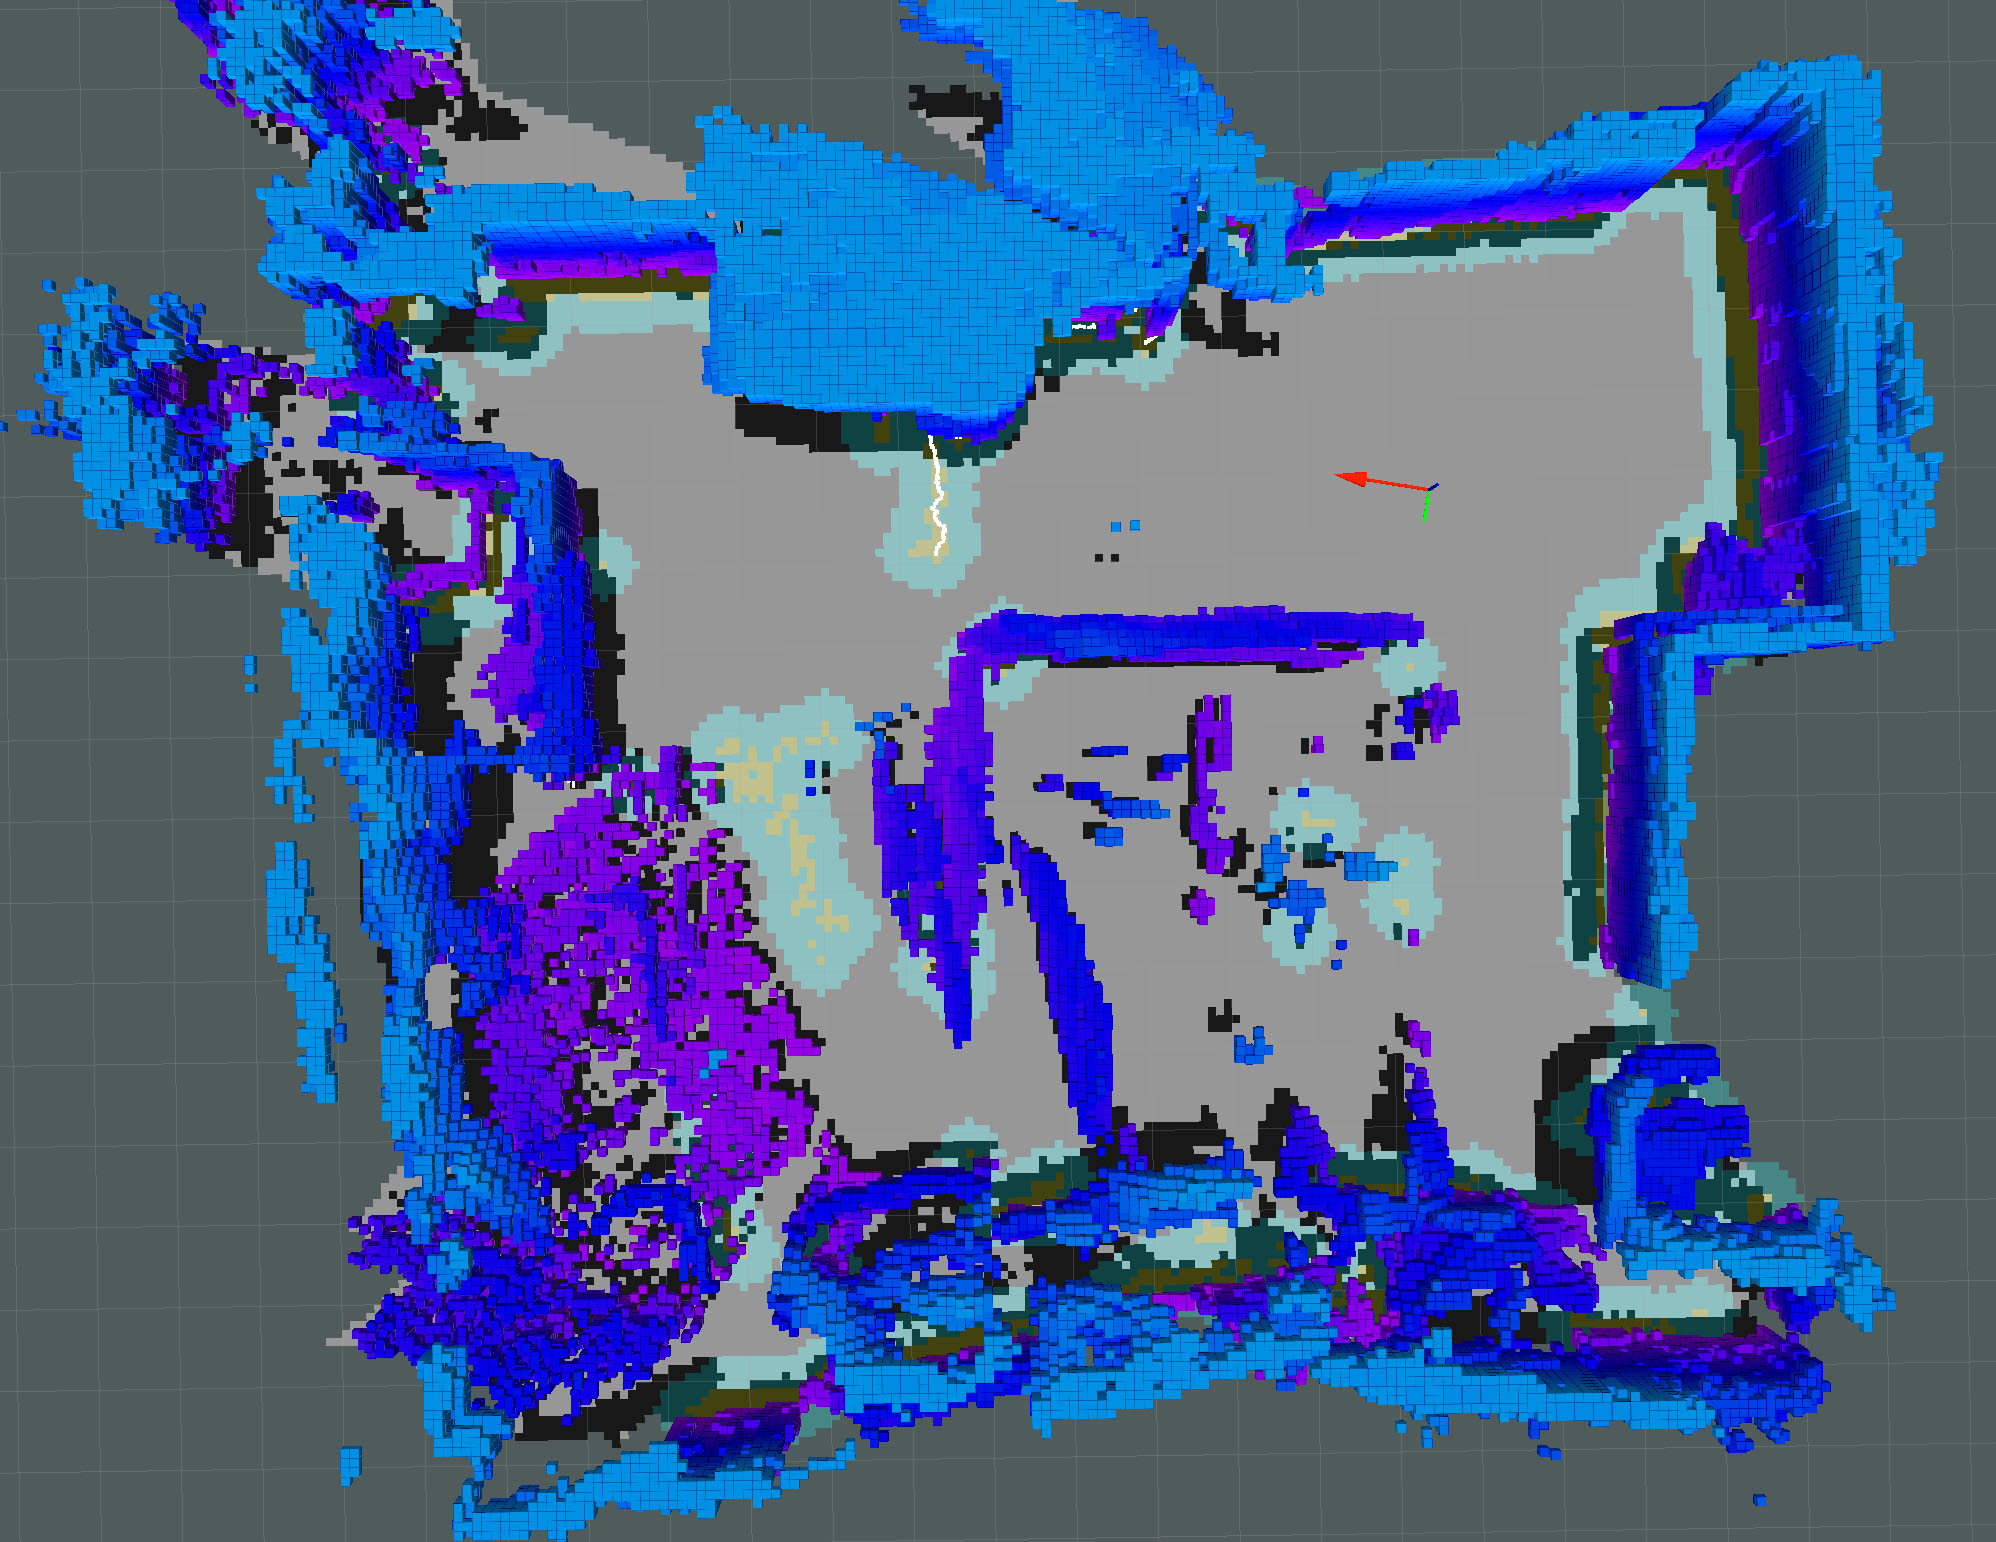
\includegraphics[width=16cm]{eval_map3.jpg}
	\caption{A display of the generated map after the robot has had a tour around the environment, as provided by RViz. It can be seen that the mapping system correctly generated a reasonable facsimile of the surrounding environment, however there is a large amount of distortion due to the drift from the visual locomotory system. Additionally, a rather large patch of the floor (bottom left, specifically) has been detected as an obstacle. As an aside, a strange effect results from the mirror that sits in the corner of the environment (top left, specifically).}
	\label{fig:eval_map_room}
\end{figure}

The resulting map output for this test is shown in \autoref{fig:eval_map_room}. While the map system generated a reasonable facsimile of the surrounding environment, there were significant distortions due to the positional drift caused by the visual odometery system, particularly when the robot was rotating. Specifically, the detected walls of the environment should have been at right angles to each other but are shown to be somewhat askew. As the mapping system depends entirely on the visual odometry system for a positional fix, there is little that could have been done to solve this issue. An additional facility to localise the robot's position based on the map rather than relative motion may have been helpful in this case, as it would be able to correct for any drift.

\section{Navigation}

To test the navigation system, the following set of tests were performed. In particular, we looked to test the time taken and accuracy for the movements generated by this system when asked to reach a particular goal. To give a comparison, we would compare the results to that of those given from manual movements following an ``ideal'' path. This would require full integration and correct operations of all previous systems thus far, as the navigation system relies on all of these systems for its own operation. 

Specifically, two different sets of tests were performed. One set would test autonomous navigation on a direct path with minimal rotation whereas the other would test a more complex path involving multiple turns.

\subsection{Direct Path}

The first set of tests aimed to test the navigation system given a goal directly in front of the robots, such that no rotations were required. The target goal would be $3$m forward from the robot's starting position. At the start of each test, the control system would be reset. Once the system was ready, a goal would be set $3$m from the starting position with a forward heading using the target tool on \emph{RViz}. Time would be recorded and general accuracy observed. As a comparison, the time taken to move along the path manually using the control would be recorded. 

Dynamic obstacle avoidance would also be tested. An object---in this case a backpack as used in the previous examples---would be placed in front of the robot as it reached $1$m. How well the navigation system managed to move around this object would then be observed.

\subsubsection{Without Obstacle}

The first experiment in this set would evaluate accuracy and timing without any obstacles in the path of the robot. First, a number of manual movements were done as a control which gave a resulting average time of $36.164$s from start point to end point. Following this, tests using the navigation system were performed. These tests gave a resulting average time of $45.495$s from start point to end point, giving an average increase in time of $9.331$s. A full listing of results can be seen in \autoref{tab:eval_nav_dp_wo}.

The navigational system spends a lot of time trying to keep the robot directly on its planned path---as one would expect---but this resulted in a number of unnecessary rotations, slowing down the overall movement. Additionally, some amount of processing time is needed for the system to compute a path. These are the most likely sources of this time increase. In general, however, the motions given by the system were accurate.

\subsubsection{With Obstacle}

The second experiment in this set would evaluate the accuracy and timing of the navigational system, but this time after an obstacle had been placed in front of the robot while it was walking. As before, a number of manual movements were performed for control---assuming that an ideal path was to curve around the obstacle. The manual movements gave an average time of $51.136$s. Following this, tests using the navigation system alone were performed. These autonomous tests gave a resulting average time of $1$m $5.677$s from start point to end point, giving an average increase in time of $14.541$s. A full listing of results can be seen in \autoref{tab:eval_nav_dp}.

\begin{figure}[h]
	\centering
	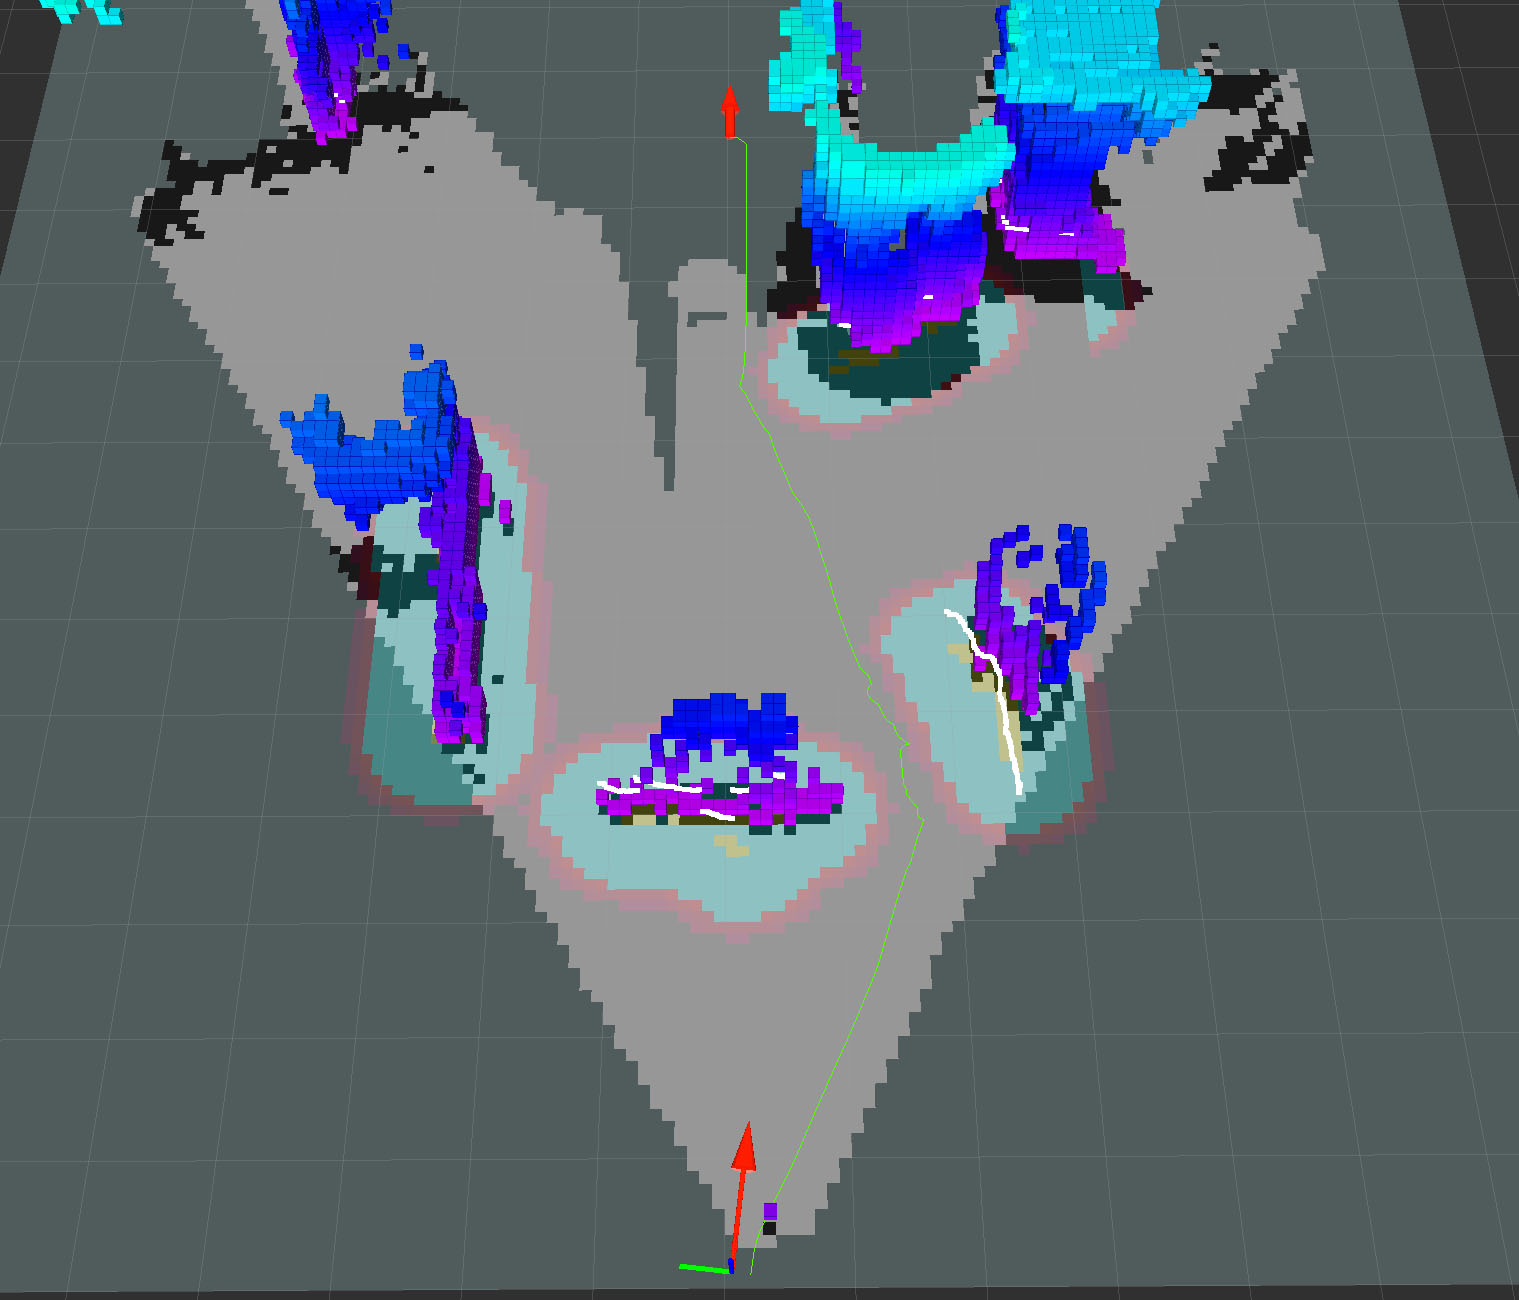
\includegraphics[width=14cm]{eval_nav.jpg}
	\caption{A display of the planned path from the autonomous navigation system after an obstacle---in this case a backpack as before---has been placed in front of the robot. Prior to this image the planned path was directly ahead with no rotations. However, after the obstacle has been placed in front of the robot, the navigation system automatically recalculates the path such that it avoid the obstacles. The circular patterns on the ground plane indicate obstacle radii on the planner's avoidance costmap.}
	\label{fig:eval_nav}
\end{figure}

An example of the path generated after the bag has been placed in front of the robot can be seen in \autoref{fig:eval_nav}. The causes of this time increase were similar to those mentioned in the previous test, but with the added rotational visual odometry drift. This rotational drift from the causes the navigation system to try and correct itself unnecessarily even though it is already in the correct position. Regardless, the robot was able to navigate around the bag successfully each time.

\subsection{Complex Path}

The second set of tests aimed to test the navigation system given a goal that would create a complex path. In these cases, the starting position and target end position would be those shown in \autoref{fig:eval_map_room}. This would show that the robot was capable of moving from one side of the room to the other. Two tests would be performed: one where the robot had a chance to move around before hand such that the environment was already mapped, and the other where the robot had no knowledge of the environment before hand. As before, time would be recorded and general accuracy observed. A manually controlled walk would be done for time comparison.

\subsubsection{Known Environment}

The first experiment in this set would aim to prove the accuracy and efficiency of the navigation system in a known environment. A number of manual tours around the ``ideal'' path would be performed before hand to get a control on timing as well as to provide a good mapping of the environment. After this, the robot would be placed at its starting position and commanded to navigate to the end position, as shown on \autoref{fig:eval_map_room}.

The manual movements from this experiment gave an average time of $2$m $5.649$s. For the autonomous navigation tests, the resulting average time was $2$m $34.014$s giving a difference of $28.365$s. This additional time is for the same reasons as explained in the previous tests. In one case, the test did not finish due to a cascading set of failures. Specifically, the navigational system managed to propel the robot into a nearby obstacle whereupon the visual odometry system ceased to give a positional fix. This required a full restart of the control system, and thus was counted as a ``did not finish'' result.

Generally, however, the test was successful. The visual odometry drift issue was still apparent overall but not enough to cause any significant problems.

\subsubsection{Unknown Environment}

The final experiment would aim to prove the accuracy and efficiency of the navigation system in an unknown environment. Unlike the previous test, no manual walking was performed to provide any mapping information. The control system would be started cleanly and then be expected to navigate from one side of the environment to the other. Manual timing information from the previous experiment would be used as a control---it did not make much sense for us to run the test manually when we already knew the environment. The navigational system would have to detect and avoid obstacles to get to the end position as it moved the robot around. 

Results from this test were varied. Out of the seven tests that completed successfully, the average time taken was $3$m $37.486$s giving a time difference from the control of $1$m $31.837$s. For those tests that did not complete successfully, similar issues as of those in the previous experiment occurred. Upon receiving the target goal, the navigational system immediately assumes it can get there directly as it has no information telling it otherwise. In these failure cases, the robot would get stuck looking at the obstacle as the visual odometry system fails to detect any features in the obstacle, causing a cascading failure of the mapping and navigational systems. In most cases, however, the robot was able to detect and adjust its path accordingly before it could get stuck.

Further tweaking of both the navigation and visual odometry systems is needed to improve these results.